\documentclass[twocolumn,a4paper]{paper}
\usepackage{graphicx}
\usepackage{siunitx}
\usepackage[super,sort&compress,comma]{natbib}
\usepackage{hyperref}
\usepackage{xr}
\externaldocument{si}


\title{Bayesian determination of the effect of a deep eutectic solvent on the structure of lipid monolayers}
\author{A.~R.~McCluskey,\textit{$^{ab}$}$^{\ddag}$ A.~Sanchez-Fernandez,\textit{$^{ac}$}$^{\ddag\P}$ K.~J.~Edler,\textit{$^{a}$}$^{\ast}$ \\
S.~C.~Parker,\textit{$^{a}$} A.~J.~Jackson,\textit{$^{cd}$} R.~A.~Campbell,\textit{$^{ef}$} and T.~Arnold \textit{$^{abcg}$}$^{\ast}$}

\institution{${a}$~Department of Chemistry, University of Bath, Claverton Down, Bath, BA2 7AY, UK. \\
${b}$~Diamond Light Source, Harwell Campus, Didcot, OX11 0DE, UK. \\
${c}$~European Spallation Source, SE-211 00 Lund, Sweden. \\
${d}$~Department of Physical Chemistry, Lund University, SE-211 00 Lund, Sweden. \\
${e}$~Institut Laue-Langevin, 71 avenue des Martyrs, 38000, Grenoble, France. \\
${f}$~Division of Pharmacy and Optometry, University of Manchester, Manchester, \\
M13 9PT, UK. \\
${g}$~ISIS Neutron and Muon Source, Science and Technology Facilities Council, \\
Rutherford Appleton Laboratory, Harwell Oxford, Didcot OX11 0QX, UK. \\
${\P}$~Present address: Department of Food Technology, Lund University, SE-211 00 \\
Lund, Sweden. \\
$\ddag$~These authors have contributed equally to the work presented within. \\
$\ast$~k.edler@bath.ac.uk; tom.arnold@esss.se}

\date{\today}

\begin{document}

\maketitle

\begin{abstract}
Deep eutectic solvents present a novel class of non-aqueous room temperature solvent with tunable properties, that are capable of promoting the self-assembly of surfactant molecules.
However, the solvation model in these systems still challenges the classic understanding of amphiphilicity.
In this work, we present the first example of the self-assembly of phospholipid monolayers at the interface between air and a non-aqueous solvent.
We use novel, chemically-consistent Bayesian modelling of X-ray and neutron reflectometry measurements to show that these monolayers broadly behave as they do on water.
However, the ability of the deep eutectic solvent to interact with the phosphatidylglycerol lipid head, leads to an apparent increase in its volume compared to that observed in water.
No such change was observed for the phosphocholine head, indicating that such interactions are head, and therefore solvent, specific.
\begin{description}
\item[Usage]
Electronic Supplementary Information (ESI) available: All analysis/plotting scripts and figure files, allowing for a fully reproducible, and automated, analysis workflow for the work presented is available at \url{https://github.com/arm61/lipids_at_airdes} (DOI: **some doi**) under an MIT license. Reduced experimental datasets are available at \url{https://researchdata.bath.ac.uk/id/eprint/548}, under a CC-BY 4.0 license.
\end{description}
\end{abstract}


Deep eutectic solvents (DES) are green, sustainable liquids that are obtained through the combination of ionic species with compounds that act as hydrogen bond donors, such as sugars, alcohols, amines, and carboxylic acids\cite{Smith2014,Dai2013,Jiang2018}.
The resulting extensive hydrogen bonding network is able to stabilise the ionic species and allows the eutectic mixture to remain liquid at room temperature\cite{Hammond2016,Hammond2017,Araujo2017,Faraone2018}.
Through different combinations of the precursor materials, it is possible to tune the solvent's physicochemical properties, such as polarity\cite{Pandey2014}, viscosity and surface tension\cite{Smith2014}, network charge\cite{Zahn2016}, and hydrophobicity\cite{Ribeiro2015,vanOsch2015}.
Recently DES have also been shown to exhibit a "solvophobic" effect through the promotion of surfactant micelle formation\cite{Sanchez-Fernandez2016,Arnold2015,Hsieh2018,Banjare2018}, phospholipid bilayer formation\cite{Bryant2017,Bryant2016,Gutierrez2009}, and the ability to stabilise non-ionic polymer\cite{Sapir2016} and protein conformations\cite{Sanchez-Fernandez2017}.

Phospholipid monolayers at the air/water interface have been widely studied as simplistic models for biological membranes.
As such, they have been used to gain insight into many biological processes that are technologically and medically relevant.
Investigations at the air/salt-water interface have identified the importance that interactions between charged phospholipid heads and ions present in solution have on the structure, monomer packing and stability of the monolayer\cite{Mohwald1990,Kewalramani2010}.
However, the native environment for lipids in-vivo is far from a simple aqueous solution.
In fact, it has been suggested\cite{Choi2011,Hammond2017} that DES effectively form within the crowded cellular environment and could assist in solubilizing biological species in an intermediate environment between that of the hydrophobic phospholipid tails and highly polar water rich regions, particularly assisting survival under extreme conditions such as freezing temperatures or drought where the water content of cells is restricted.
Despite the broad interest in these systems, the presence of stable phospholipid monolayers at the interface between air and any non-aqueous media has not been previously reported, to the best of the authors' knowledge.

This work presents the first investigation of the structure of phospholipid monolayers at an air-DES interface.
We have used a chemically-consistent approach to model X-ray (XRR) and neutron (NR) reflectometry measurements and thereby evaluate the effect of this non-aqueous solvent on the structure of phospholipid monolayers.

Recent developments in computational resources and software have enabled powerful methodologies and algorithms to be harnessed by those from non-expert backgrounds.
This has benefitted significantly from open-source software projects such as the Python language\cite{vanRossum1995} and the Jupyter notebooks framework\cite{Kluyver2016}.
In the area of NR and XRR, the landscape of data-analysis software is diverse, with a range of software packages available from a variety of sources; refnx\cite{Nelson2018}, MOTOFIT\cite{Nelson2006}, Rascal\cite{HughesRascal} Aurore\cite{Gerelli2016}, and GenX\cite{Bjorck2007}.

The use of a Python library, such as refnx, enables the implementation custom models that contain chemically-relevant information as well as the application of probability distribution function (PDF) sampling techniques.
The Python library emcee\cite{Foreman-Mackey2013} offers refnx to access the Goodman \& Weare Affine Invariant Markov chain Monte Carlo (MCMC) Ensemble method\cite{Goodman2010}.
This allows the sampling of the high-dimensionality parameter space, relevant in reflectomety analysis, in a Bayesian fashion, where the new samples are generated with consideration of those sampled previously\cite{Sivia2006}.
Bayesian inference gives an understanding of the PDF for the fitted parameters and therefore estimations of their inverse uncertainties and inter-parameter correlations.

%
\begin{figure}
\centering
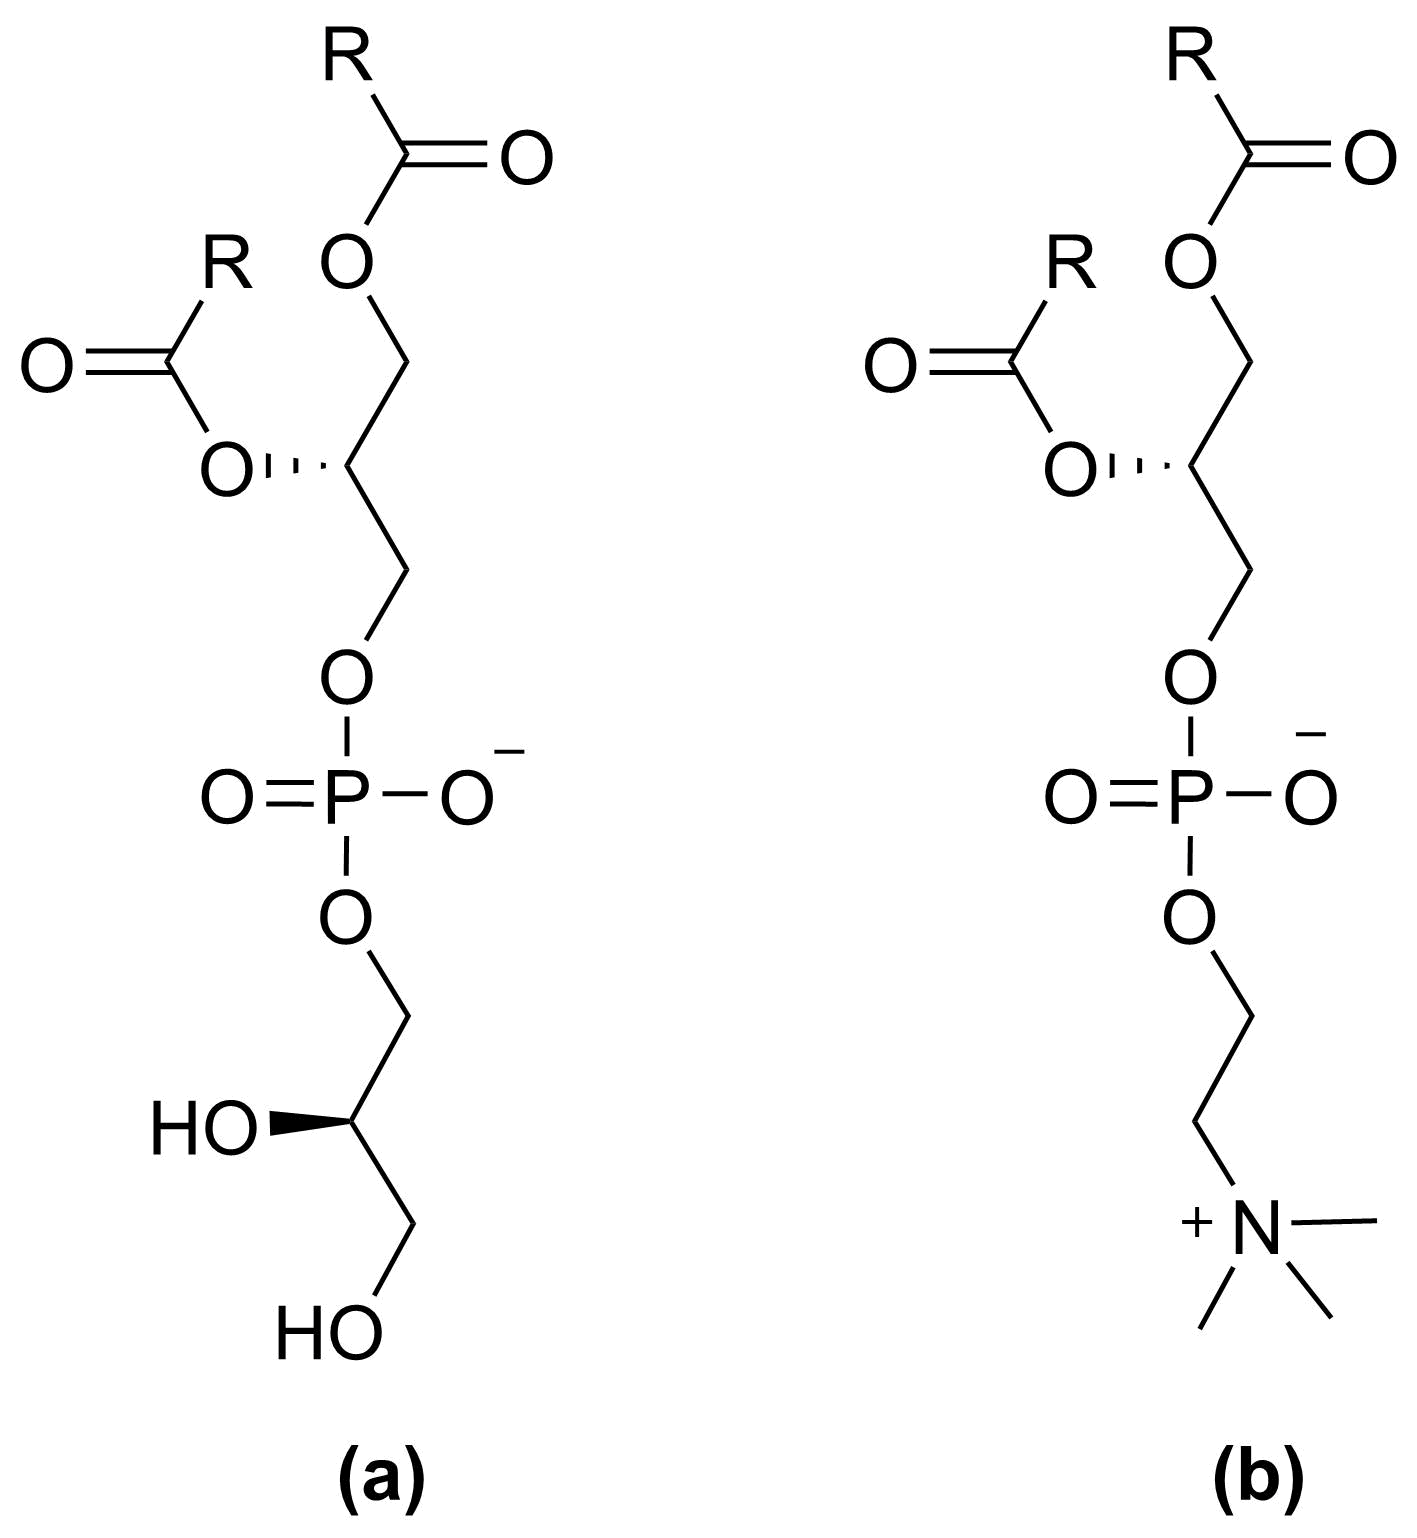
\includegraphics[width=0.3\textwidth]{figures/head_groups}
\caption{\label{fig:heads}\small The two lipid classes with different head groups compared in this study, where R indicates the hydrocarbon tail; (a) phosphatidylglycerol (PG), (b) phosphocholine (PC).}
\end{figure}
%
We developed a chemically-consistent model (detail in the ESI) that allowed for the co-refinement of reflectometry measurements at different surface concentration.
The model was applied to the study of four phospholipids monolayers, namely 1,2-dipalmitoyl-sn-glycero-3-phosphocholine (DPPC, C$_{16}$ tails), 1,2-dimyristoyl-sn-glycero-3-phosphocholine (DMPC, C$_{14}$ tails),  1,2-dilauroyl-sn-glycero-3-phosphocholine (DLPC, C$_{12}$ tails) and 1,2-dimyristoyl-sn-glycero-3-phospho-(1'-rac-glycerol) (DMPG, C$_{14}$ tails), at the air-1:2 choline choride:glycerol mixture interface, by XRR at a series of different surface pressures, between \SIrange{15}{40}{\milli\newton\per\meter}.
Unlike monolayer models applied previously\cite{Mohwald1990,Kewalramani2010,Bayerl1990,Johnson1991,Clifton2012,Helm1987,Daillant1990}, our model made no assumption of the volume of the lipid head, $V_h$, or tail, $V_t$.
Instead these parameters, along with the thickness of the phospholipid head layer, $d_h$, were allowed to vary for each lipid.
However, their values were constrained to be self-consistent for a single lipid over multiple measurements at different surface pressures.

This model was required, despite the general consensus that the volume of the phosphocholine (PC) head is \SIrange{320}{360}{\cubic\angstrom}, while the phosphatidylglycerol (PG) head is \SIrange{289}{291}{\cubic\angstrom} (see Table \ref{tab:water}), since the DES may affect the head volume, because of differing electrostatic interactions compared to water.
Furthermore, it is known that, on water, increased surface pressure and associated liquid-expanded to liquid-condensed (LE-LC) phase transitions lead to a compression of the lipid tail volume\cite{Marsh2010,Small1984}.
It has been shown recently that such hydrocarbon compaction should be included when modelling reflectometry data\cite{Campbell2018}, something that has not necessarily been accounted for the in the literature.

%
\begin{figure}
	\centering
	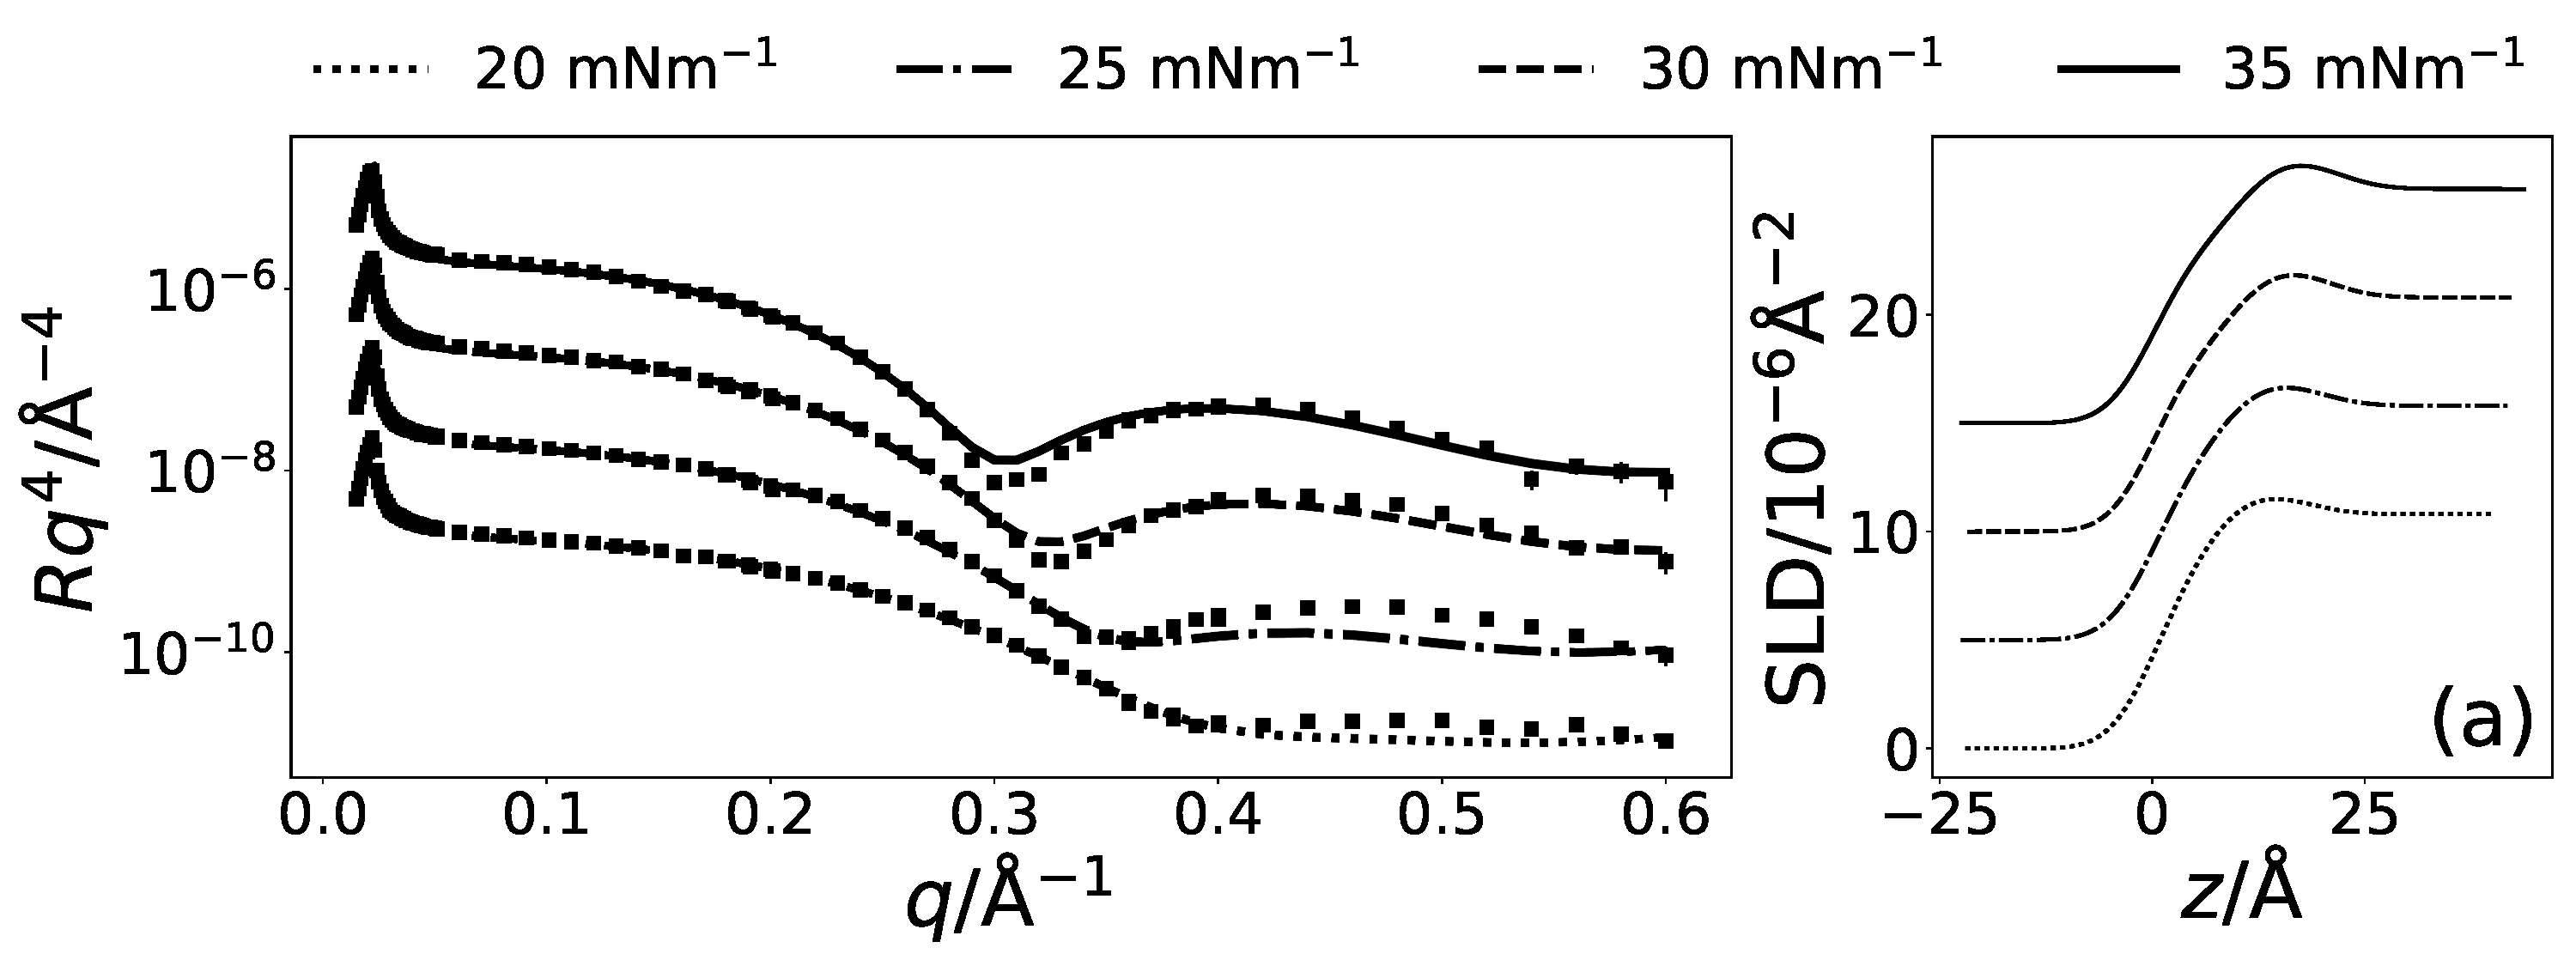
\includegraphics[width=0.45\textwidth]{figures/dlpc_ref_sld}
	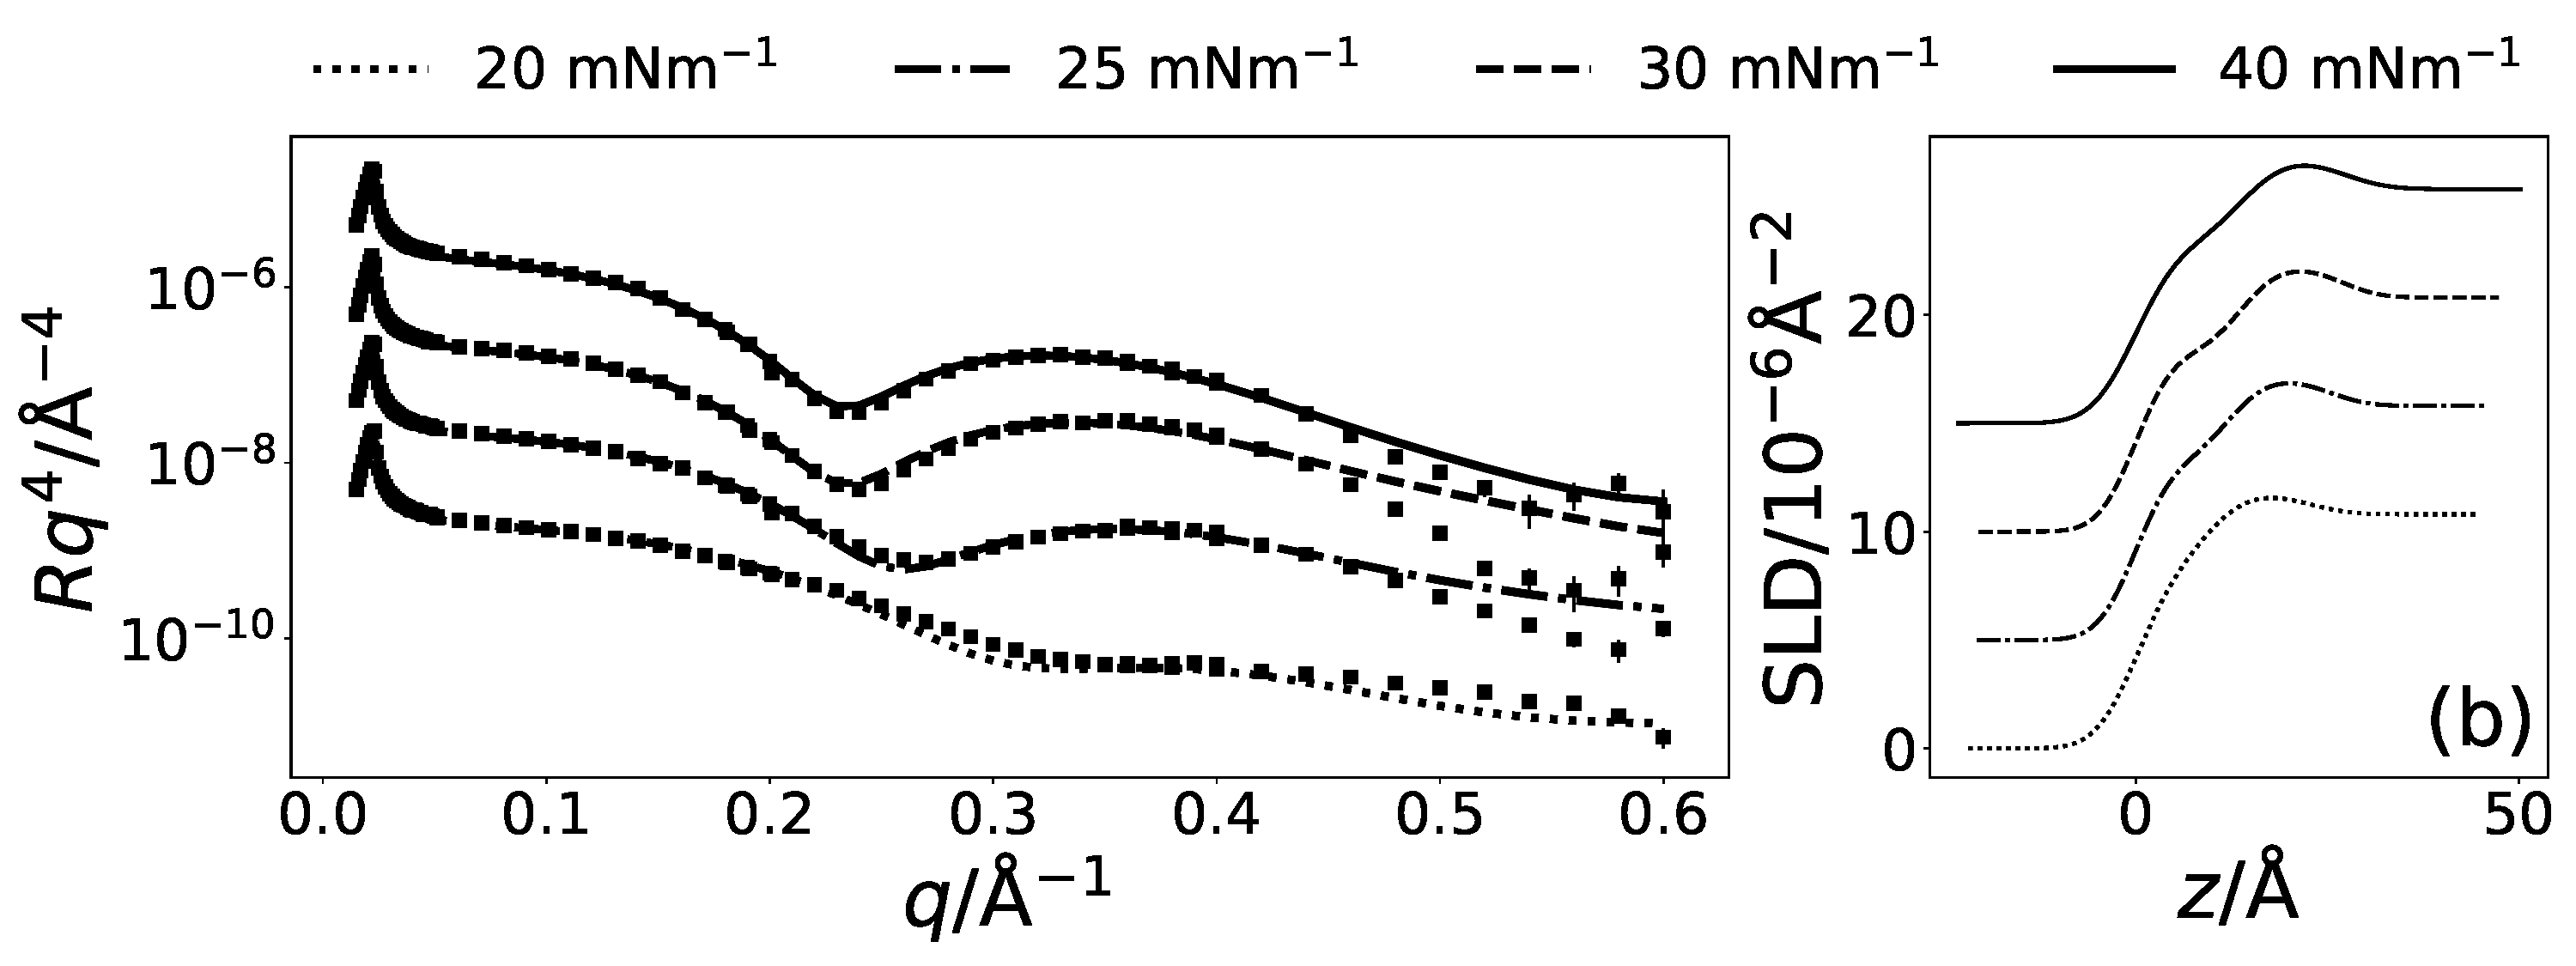
\includegraphics[width=0.45\textwidth]{figures/dmpc_ref_sld}
	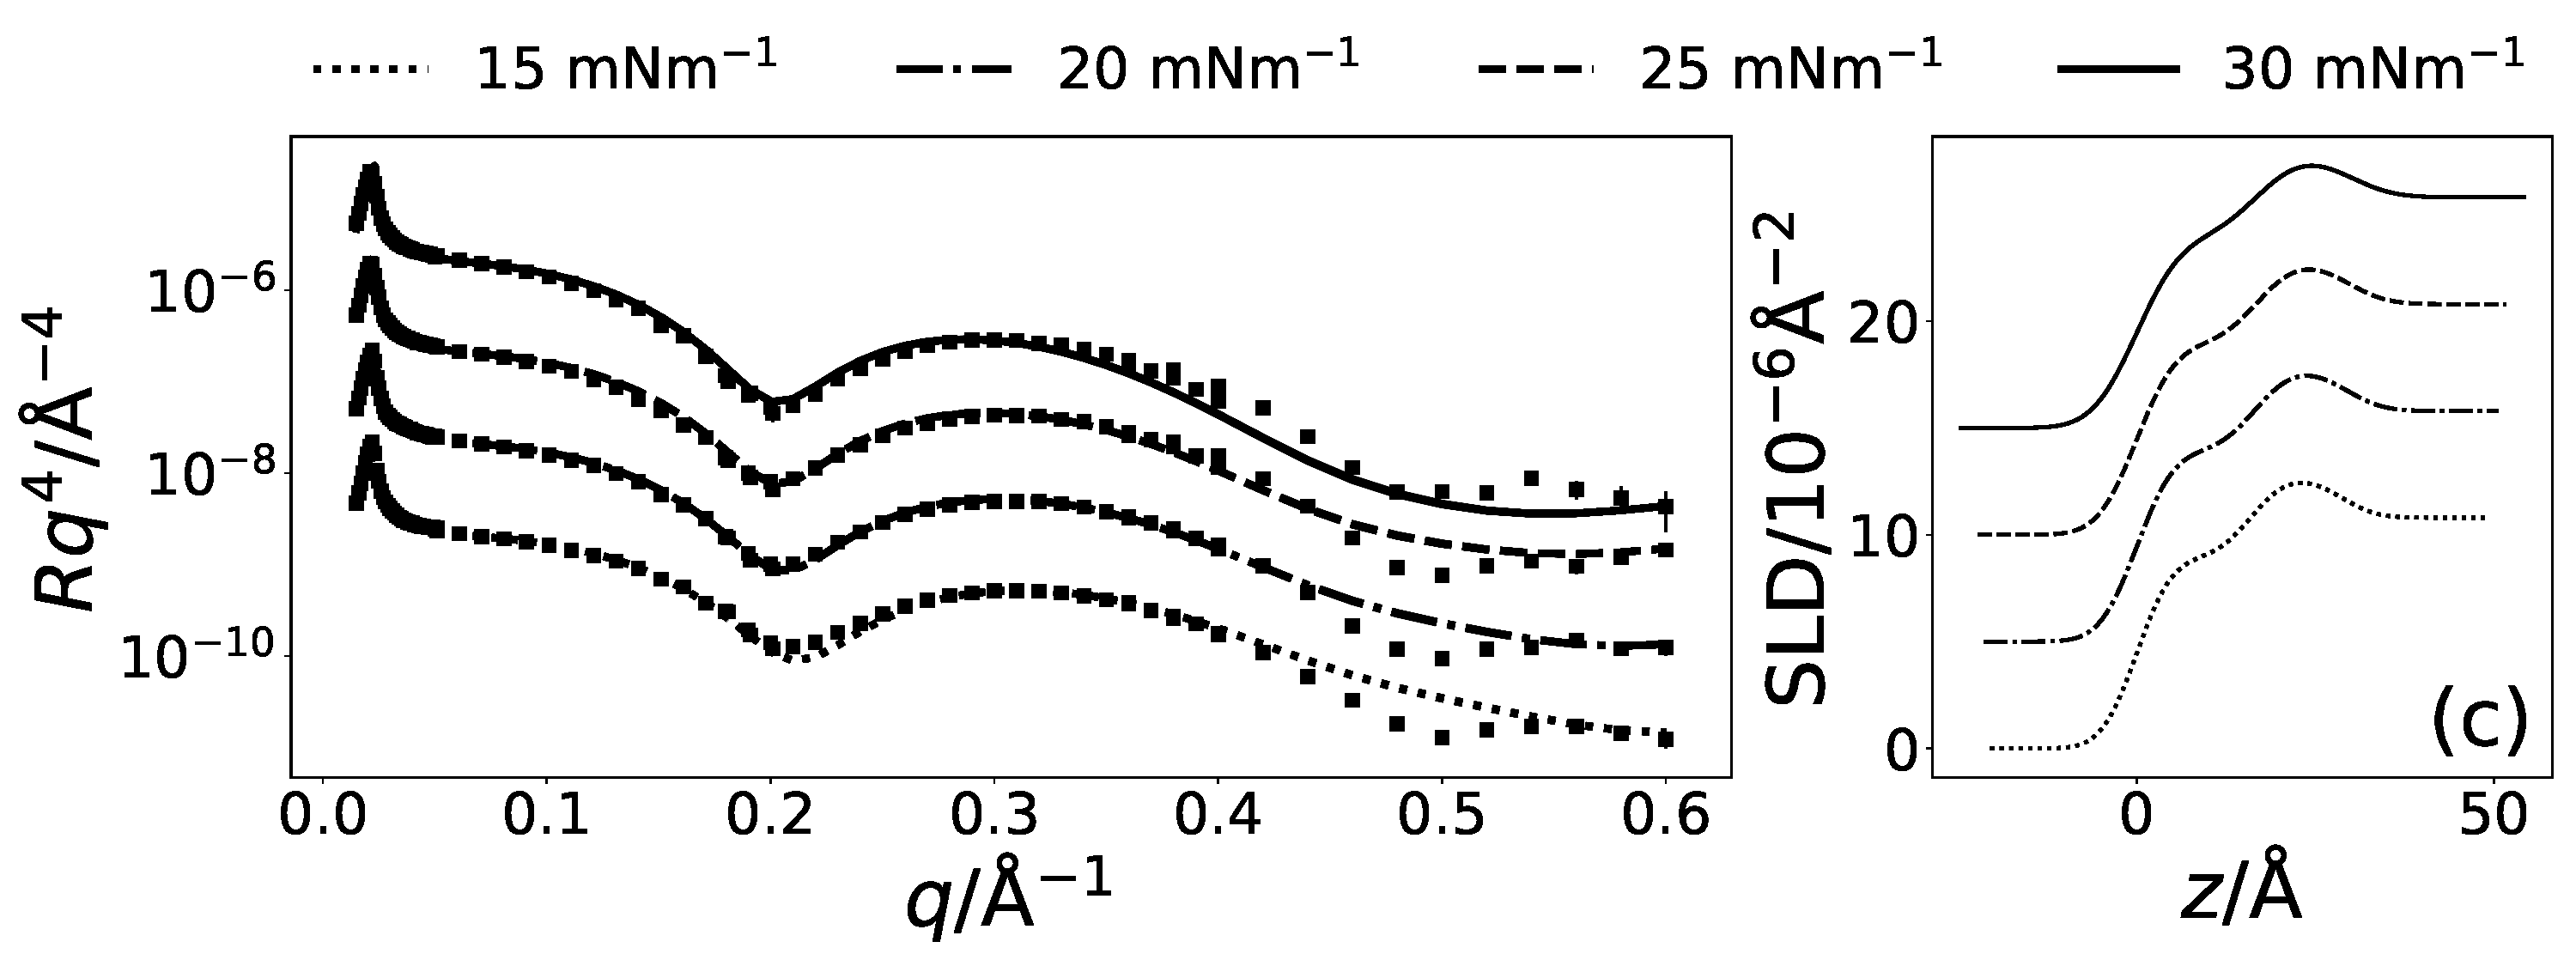
\includegraphics[width=0.45\textwidth]{figures/dppc_ref_sld}
	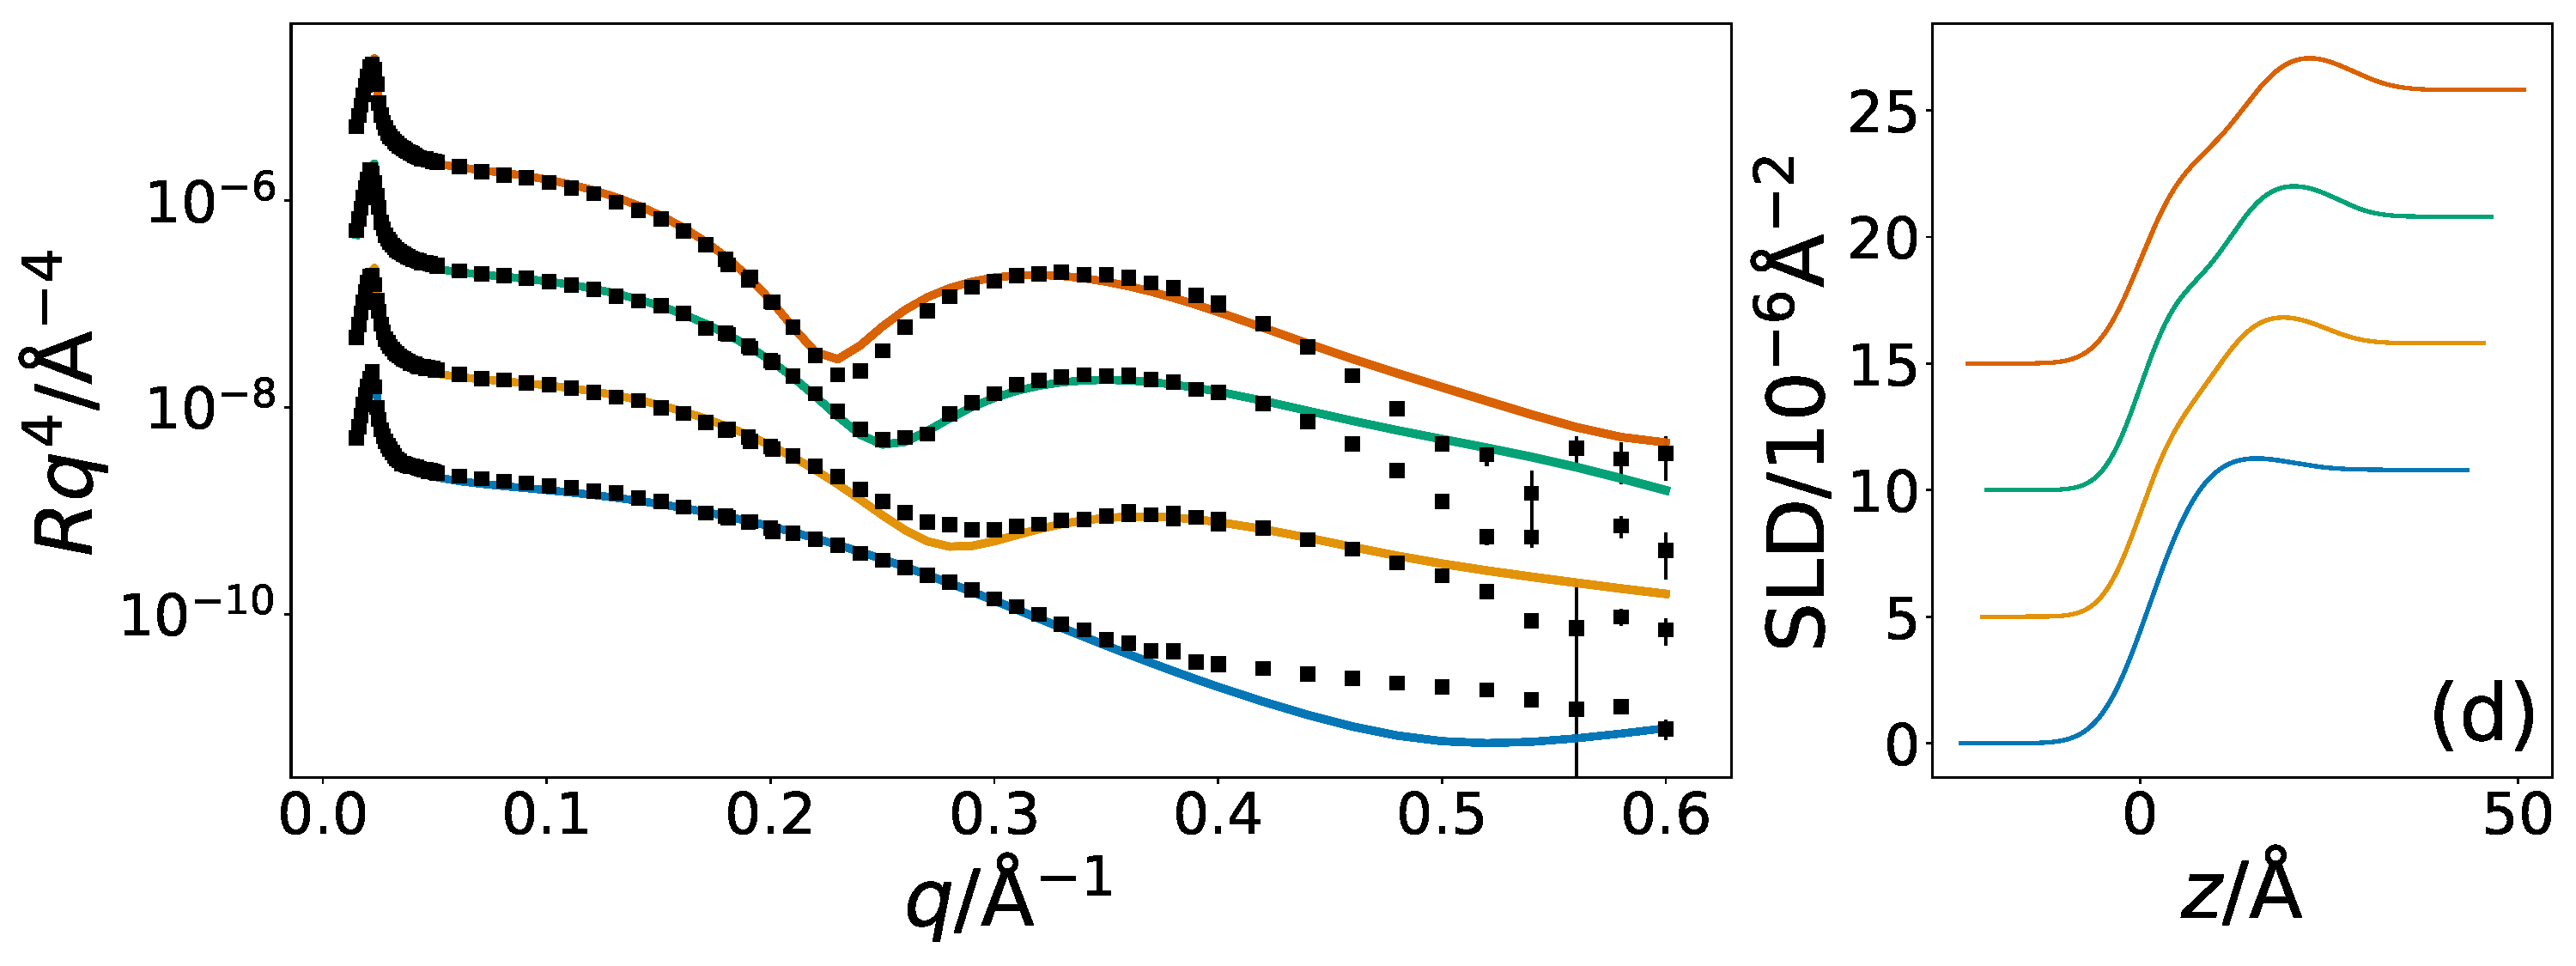
\includegraphics[width=0.45\textwidth]{figures/dmpg_ref_sld}
	\caption{\small The XRR profiles (left) and SLD profiles (right) for each of the four lipids; (a) DLPC, (b) DMPC, (c) DPPC, (d) DMPG, at the four measured surface pressures; see legend above each plot. The different surface pressure XRR profiles have been offset in the $y$-axis by an order of magnitude and SLD profiles offset in the $y$-axis by \SI{5e-6}{\per\square\angstrom}, for clarity.}
	\label{fig:lipids}
\end{figure}
%

The custom model for each lipid, based on the standard two-layer model widely used for lipids on water, was first fitted to the experimental XRR data, and the associated SLD profiles are shown in Figure \ref{fig:lipids}.
Table \ref{tab:liptab} presents the mean value, and asymmetric uncertainies that correspond to a \SI{95}{\percent} confidence interval, for the PDF for each of the varying parameters; the tail tilt angle, $\theta_t$, the interfacial roughness, $\sigma$, the head and tail volumes, $V_h$ and $V_t$ respectively, and the head layer thickness, $d_h$.
In order to constrain the fitting process only $\theta_t$ and $\sigma$ were allowed to vary independently of surface pressure. The other parameters, $V_h$, $V_t$ and $d_h$ were fitted to a single value for all of the surface pressures measured for each lipid.

%
\begin{table*}
  \centering
	\caption{\label{tab:liptab}\small The best-fit values, and associated 95 \% confidence intervals for the varying parameters in the XRR models, at the highest surface pressure (SP) measured. The values of $d_t$ were found from the appropriate values of $\theta_t$ using Eqn. \ref{equ:tl} and the values for $\phi_h$ were obtained from the appropriate use of Eqn. \ref{equ:phih}.}
	\begin{tabular}{ccccc}
		Lipid & DLPC & DMPC & DPPC & DMPG \\
    SP/\si{\milli\newton\per\meter} & 35 & 40 & 30 & 30 \\
		\hline
		$\theta_t$/\si{\degree} & \input{../output/dlpc/angle35.txt} & \input{../output/dmpc/angle40.txt} & \input{../output/dppc/angle30.txt} & \input{../output/dmpg/angle30.txt} \\
		$\sigma$/\si{\angstrom} & \input{../output/dlpc/rough35.txt} & \input{../output/dmpc/rough40.txt} & \input{../output/dppc/rough30.txt} & \input{../output/dmpg/rough30.txt} \\
    \hline
    $V_t$/\si{\cubic\angstrom} & \input{../output/dlpc/vt.txt} & \input{../output/dmpc/vt.txt} & \input{../output/dppc/vt.txt} & \input{../output/dmpg/vt.txt} \\
		$V_h$/\si{\cubic\angstrom} & \input{../output/dlpc/vh.txt} & \input{../output/dmpc/vh.txt} & \input{../output/dppc/vh.txt} & \input{../output/dmpg/vh.txt} \\
		$d_h$/\si{\angstrom} & \input{../output/dlpc/head.txt} & \input{../output/dmpc/head.txt} & \input{../output/dppc/head.txt} & \input{../output/dmpg/head.txt} \\
    \hline
    $\phi_h$/$\times10^{-2}$ & \input{../output/dlpc/solh35.txt} & \input{../output/dmpc/solh40.txt} & \input{../output/dppc/solh30.txt} & \input{../output/dmpg/solh30.txt} \\
		$d_t$/\si{\angstrom} & \input{../output/dlpc/tail35.txt} & \input{../output/dmpc/tail40.txt} & \input{../output/dppc/tail30.txt} & \input{../output/dmpg/tail30.txt} \\
	\end{tabular}
\end{table*}
%

In keeping with previous literature, \cite{Mohwald1990,Vaknin1991}, the tail layer thickness, $d_t$, increases with the number of hydrocarbon atoms present.
Furthermore, the thickness of the tail layers agrees well with values found for water-analogues; \input{../output/dmpc/tail30.txt}\si{\angstrom} at \SI{30}{\milli\newton\per\meter} in DES compared with $d_t=\SI{15.8}{\angstrom}$ at \SI{30}{\milli\newton\per\meter}\cite{Johnson1991} in water for DMPC, and \input{../output/dppc/tail30.txt}\si{\angstrom} at \SI{30}{\milli\newton\per\meter} in DES compared with $d_t=\SI{16.7}{\angstrom}$ at \SI{40}{\milli\newton\per\meter}\cite{Helm1987} in water for DPPC.
In all cases the surface roughness was found to be higher than in water. However this should be considered in the context that the absolute surface tension of the DES is less than water with a corresponding higher surface roughness\cite{Arnold2015}.

Figure \ref{fig:lipresults} shows the tail layer thickness increasing with surface pressure, before plateuing; for DPPC this occurs at \SI{20}{\milli\newton\per\meter}, DMPC at \SI{30}{\milli\newton\per\meter} and for DMPG and DLPC the plateu can be assumed to be at higher pressures than those studied.
This phenomenon has been noted before for DMPC\cite{Bayerl1990} and DPPC\cite{Campbell2018} at the air-water interface.

%
\begin{figure}
	\centering
	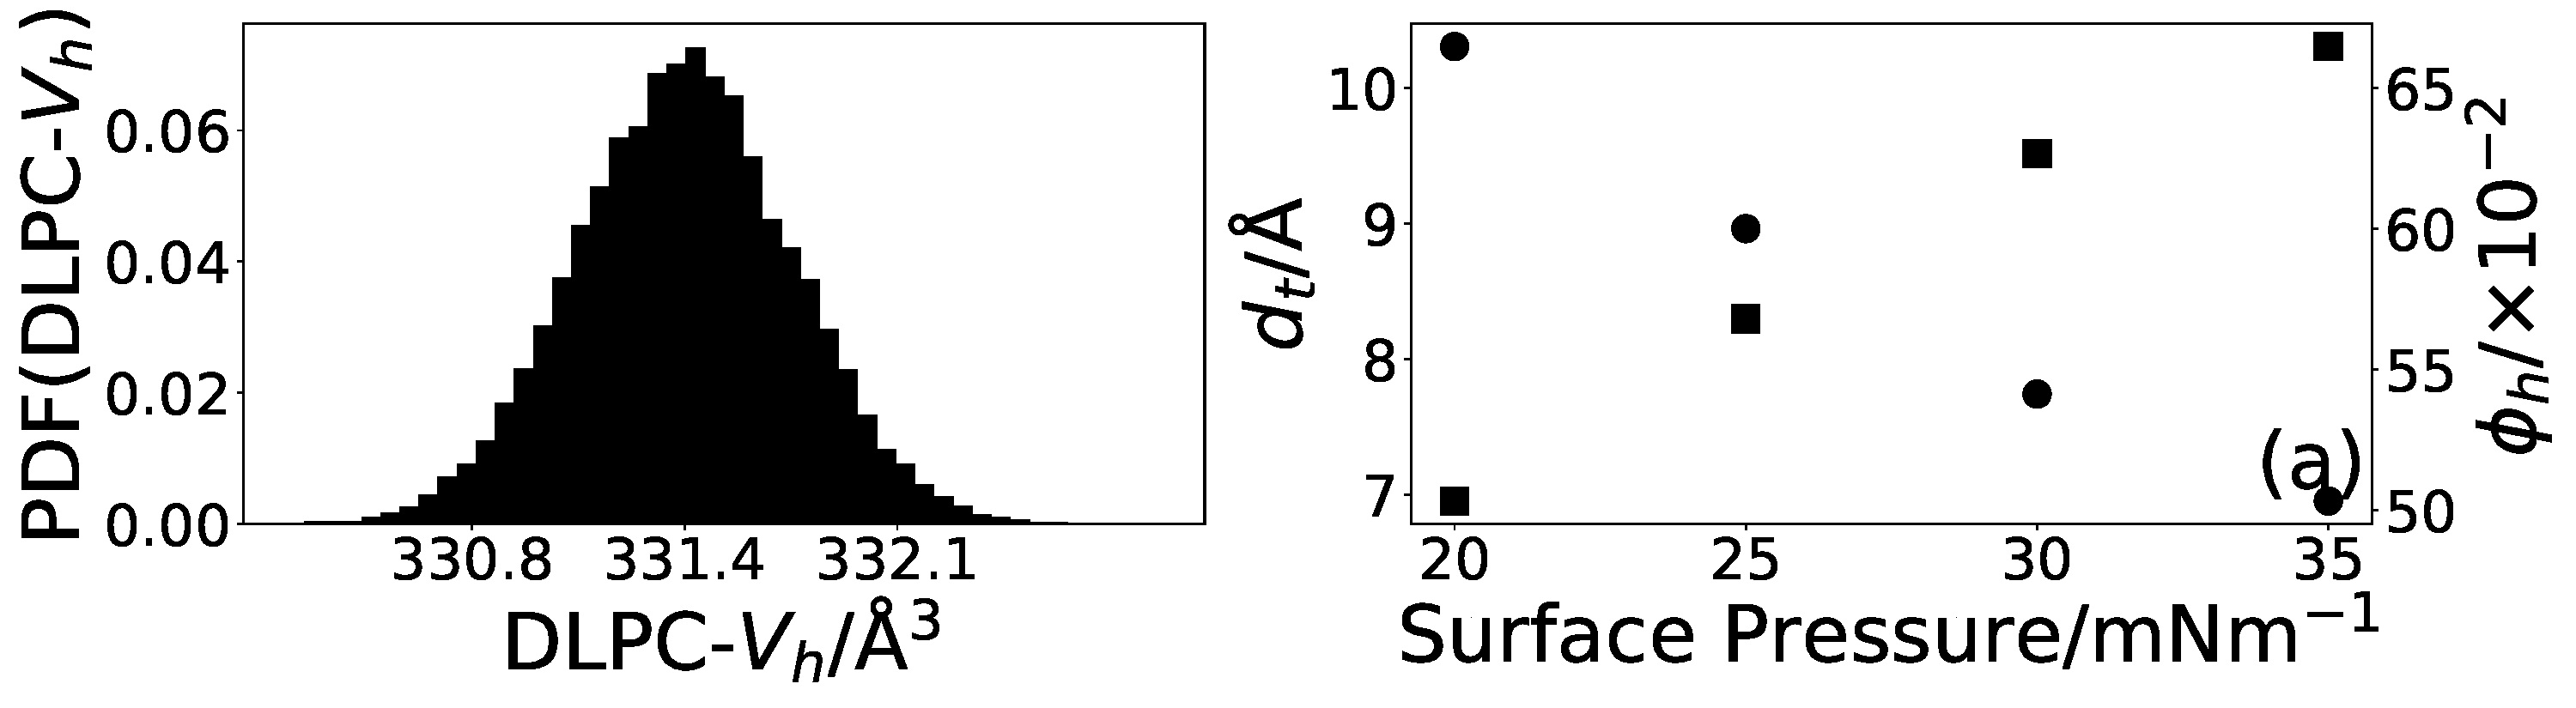
\includegraphics[width=0.45\textwidth]{figures/dlpc_vh_dt_phi}
	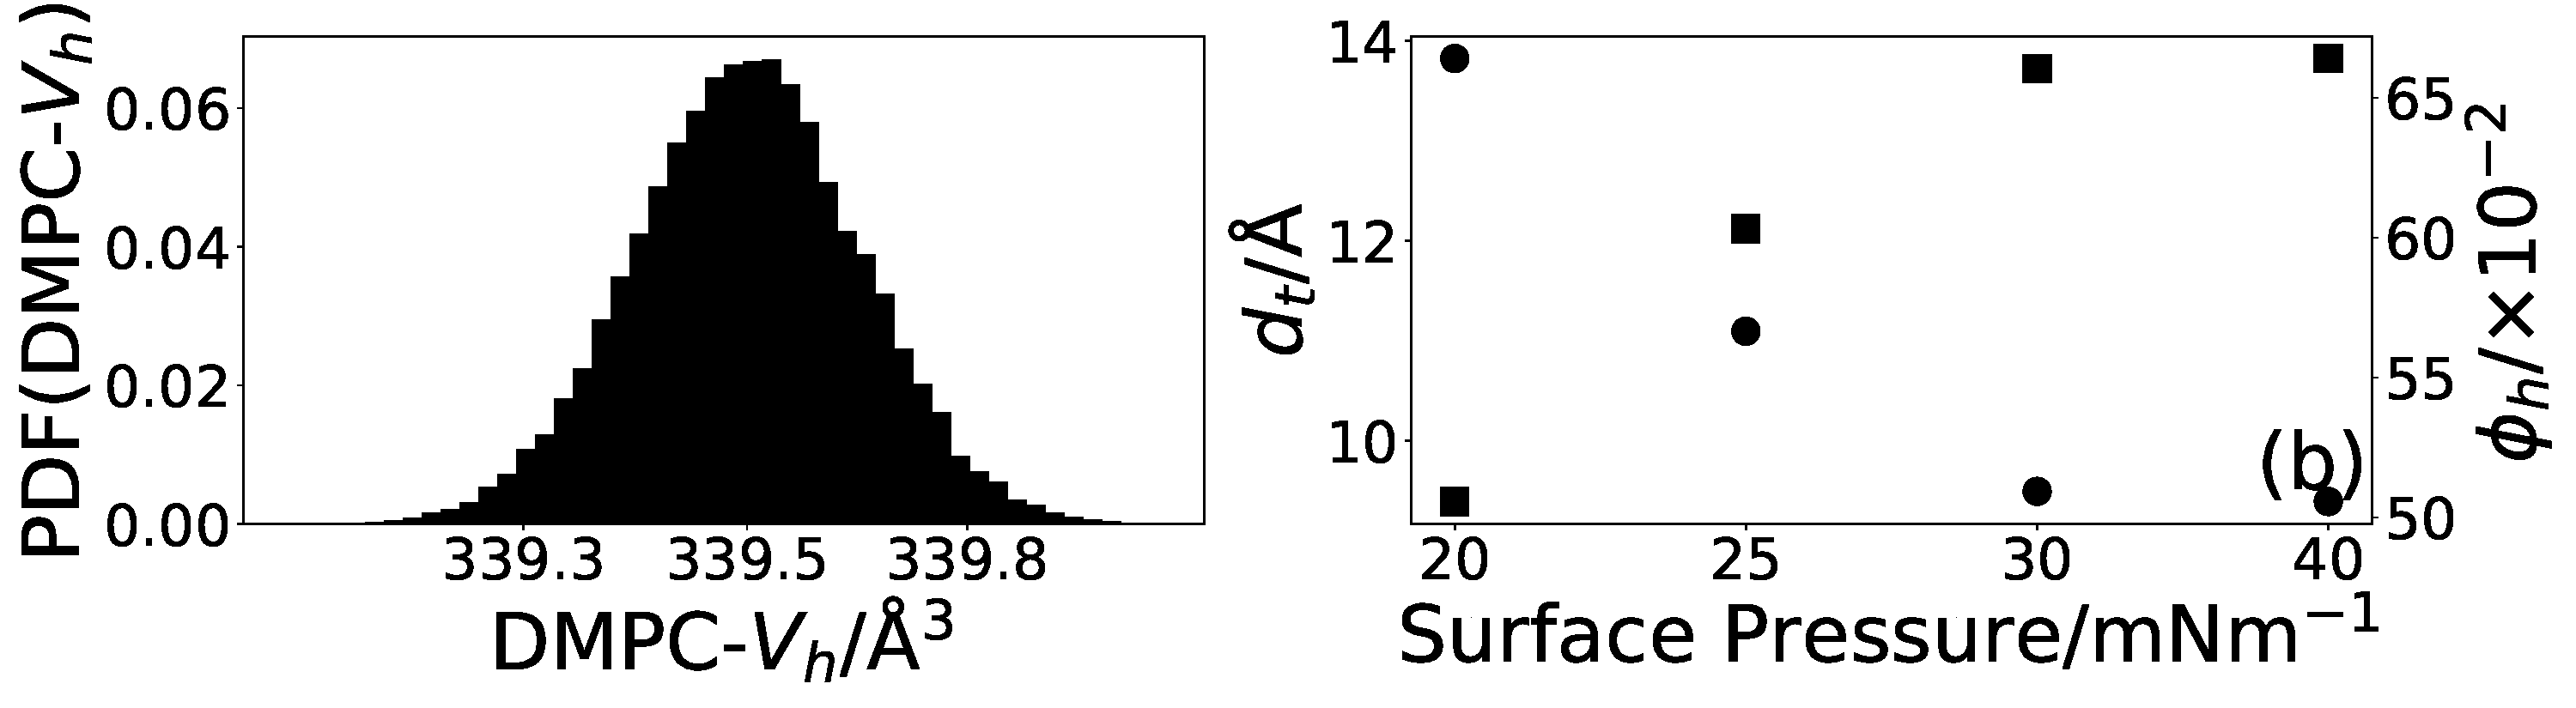
\includegraphics[width=0.45\textwidth]{figures/dmpc_vh_dt_phi}
	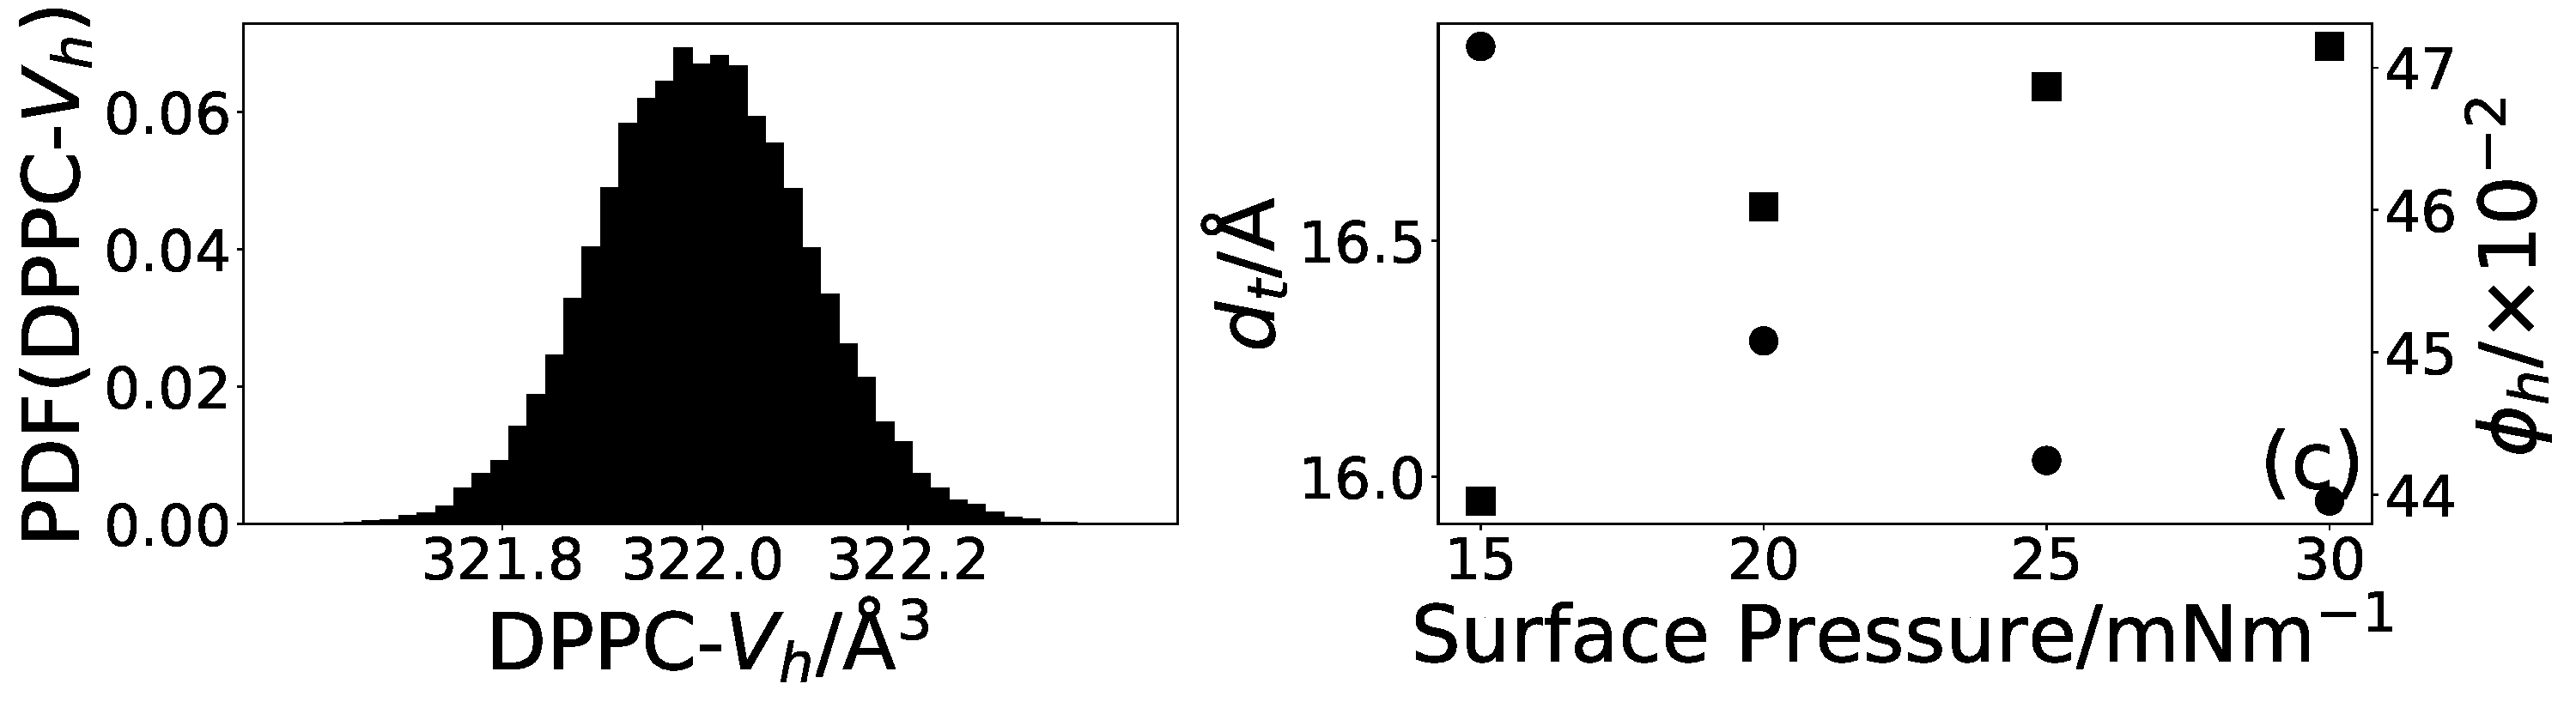
\includegraphics[width=0.45\textwidth]{figures/dppc_vh_dt_phi}
	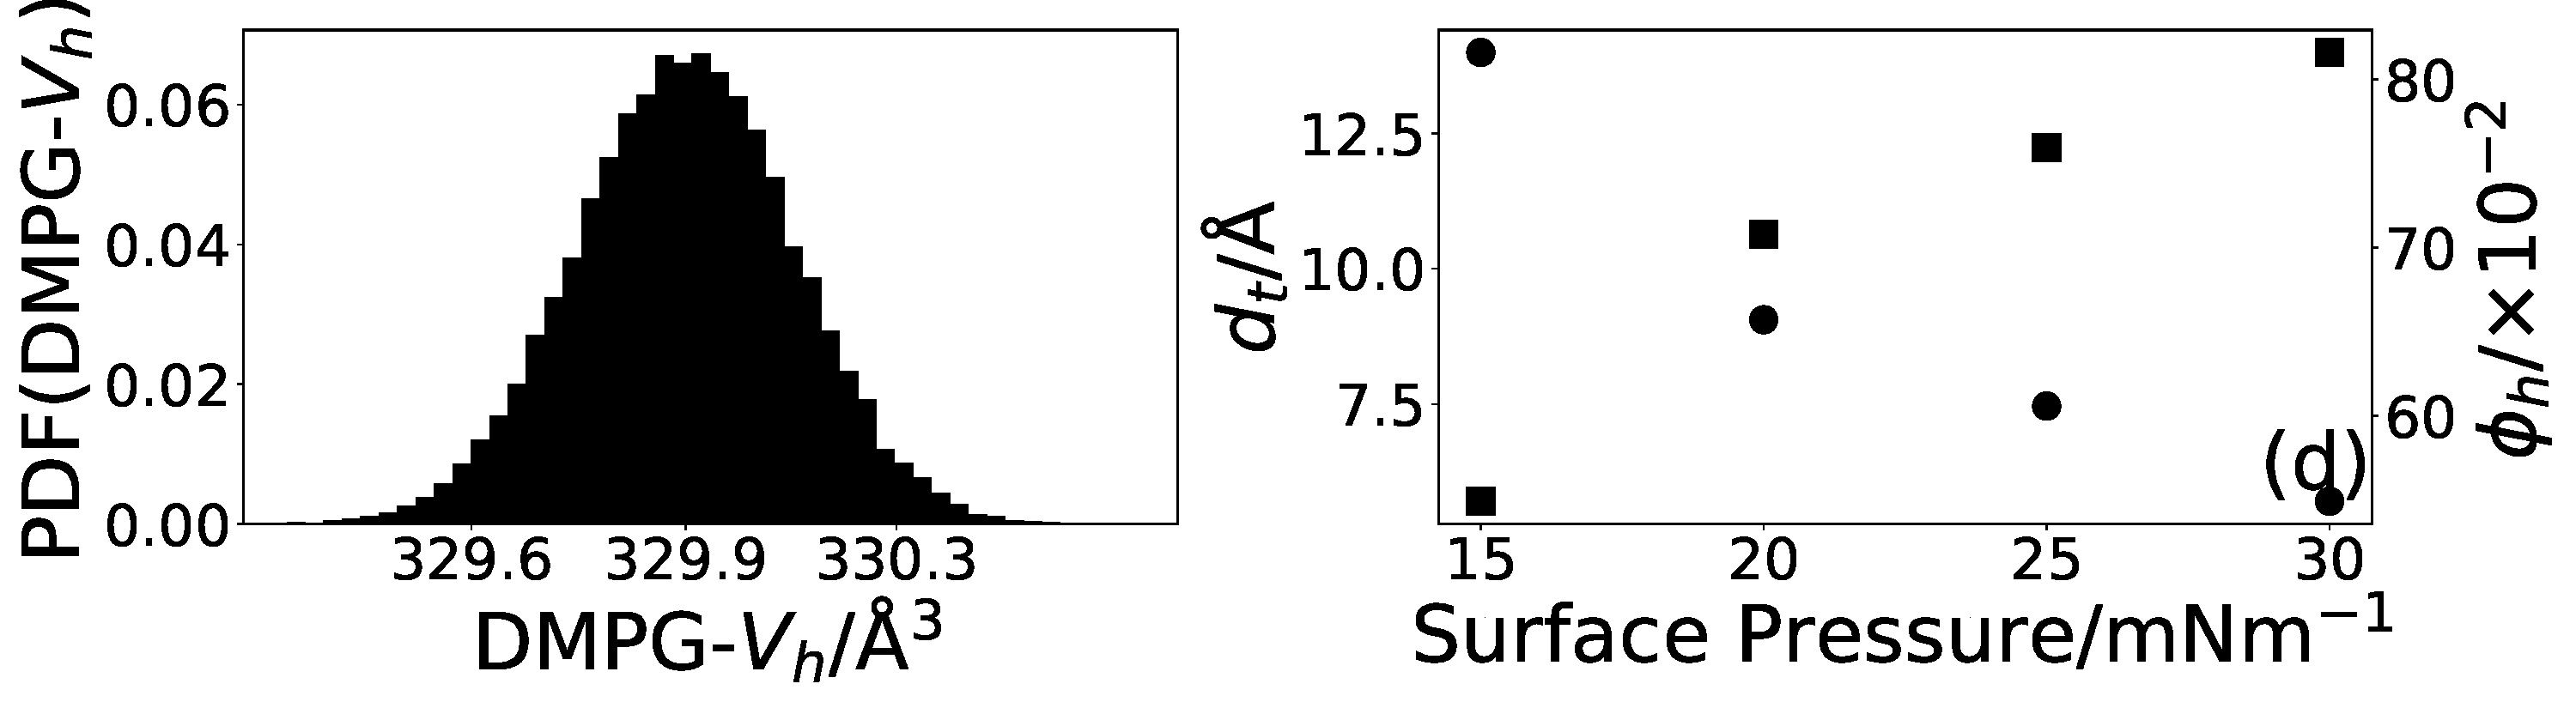
\includegraphics[width=0.45\textwidth]{figures/dmpg_vh_dt_phi}
	\caption{\small The PDFs of the head volume (left) and variation of $d_t$ (squares) and $\phi_h$ (circles) with surface pressure for each of the four lipids; (a) DLPC, (b) DMPC, (c) DPPC, (d) DMPG. The values of $d_t$ were found from the appropriate values of $\theta_t$ using Eqn. \ref{equ:tl}.}
	\label{fig:lipresults}
\end{figure}
%

In Figure \ref{fig:lipresults}, it is clear that for all four lipids, as the surface pressure is increased there is a corresponding decrease in the percentage solvent, $\phi_h$, present in the lipid head layer.
This can be rationalised by considering when the surface pressure is increased, the free volume available between the lipid heads reduces, forcing the solvent out of the lipid head layer and into the bulk.
A similar effect has been observed when increasing the surface pressure from \SI{11}{\milli\newton\per\meter} to \SI{31}{\milli\newton\per\meter} for a DMPC/DMPG monolayer at the air-water interface\cite{Bayerl1990}.

When comparing Tables \ref{tab:water} and \ref{tab:liptab} it is clear that the volume of the lipid tails are significantly lower in the current measurements than found previously, by other techniques.
It is unlikely that this is a result of the DES subphase, due to the hydrophobic nature of the lipid tails.
Such a reduction has been shown previously\cite{Campbell2018}, where it was rationalised by the compaction of the monolayer at elevated surface pressure.
In that work, the optimal value of the tail volume for DPPC was found to be \SI{772}{\cubic\angstrom} at a surface pressure of \SI{35}{\milli\newton\per\meter}, this agrees well with the value of \input{../output/dppc/vt.txt}\si{\cubic\angstrom} found in this work at surface pressures of 15, 20, 25, and \SI{30}{\milli\newton\per\meter}.
The reduction was found to be \SIrange{8}{12}{\percent} for DPPC, DMPC and DLPC when compared with literature sources at \SIrange{24}{30}{\celsius}, this is in good agreement with the maximum compression percentage of \SI{15}{\percent} noted by Small \emph{et al.}\cite{Small1984}.
DMPG shows a small increase in the tail volume relative to the literature value quoted at lower temperature.
However, our value is similar to that found for DMPC on DES, which has the same tail structure and suggests that our results are at least self-consistent.

While we have confidence that the individual surface pressures measured were reliable, we were unable to collect consistent Langmuir isotherm measurements, due to the poor wetting properties of the DES.
This inconsistency means that we cannot be confident in the phase of the lipids based on the surface pressure alone.
Instead we have used grazing incidence X-ray diffraction to confirm the phases of DMPC and DPPC at \SI{30}{\milli\newton\per\meter}.
Thus DPPC was found to be in the LC phase at room temperature while DMPC was in the LE phase at room temperature and the LC phase at 7C (see Section \ref{sec:gixd}).
This is essentially the same phase behaviour as is observed in water \cite{Phillips1968} and by considering that there is little interaction between the lipid tails and the DES we believe that it is unlikely that there is a significant change in the phase behaviour in these systems\cite{Nagle1976}.
We therefore assume that for all four surface pressures, as is the case on water, the lipids adopt the same phase for all surface pressures measured and any variation in the structure would manifest only as a change in the tail thickness, via the tail tilt angle.
This allowed a single tail volume to be fitted for each lipid at all four surface pressures that were measured.

Figure \ref{fig:lipresults} shows the PDFs for the head volume for each of the four lipids.
The three lipids with the PC head are consistent with values of around \SI{330}{\cubic\angstrom}, regardless of hydrocarbon tail.
This agrees well with the values found for the same head in water (Table \ref{tab:water}).
Interestingly, the volume for the PG head is similar to that for the PC head with a value of \input{../output/dmpg/vh.txt}\si{\cubic\angstrom}, whereas it is considered to be smaller in water when measured by either DMPG using differential vibrating tube densimetry\cite{Pan2012} (\SI{291}{\cubic\angstrom}) or POPG using molecular dynamics simulations\cite{Kucerka2012} (\SI{289}{\cubic\angstrom}).
This indicates that there may be some effect arising from the solvation in DES causing an apparent increase in the PG head volume when compared with water.

The major difference between the two heads is the fact PG head is negatively charged whereas the PC head is zwitterionic (Figure \ref{fig:heads}).
It has been shown previously that, due to the electrostatic interaction, the conformation of the PC head is folded in water\cite{Gilliams2016}.
A similar structure may occur for the PG head, with a weaker interaction between the partially postively-charged alcoholic hydrogen atoms and the negatively-charged phosphate group.
Therefore, the observed increase found for the PG volume in DES when compared with water may be due to the unfolding of the PG head, where the solvent is capable of providing a greater screening effect to the PG head than that present in water.
This may not be observed for the PC head due to the greater strength of the folding interaction arising from the formally-charged nature of the ammonium group.
It would be anticipated that this unfolding would result in an increase in the thickness of the lipid head layer.
Previously, DPPG has been reported to have a head layer thickness of \SI[separate-uncertainty=true]{10.3\pm0.4}{\angstrom} at \SI{22}{\milli\newton\per\meter} \cite{Clifton2012} and \SI[separate-uncertainty=true]{9.7\pm1.0}{\angstrom} at \SI{15}{\milli\newton\per\meter} \cite{Ciumac2017} from NR measurements, which it slightly less than the \input{../output/dmpg/head.txt}\si{\angstrom} determined in the current work, further suggesting that the unfolding of the PG head.
Previously, the presence of short range, electrostatic interactions has been noted to impact the solution structure adopted by zwitterionic surfactants in choline chloride:glycerol\cite{Sanchez-Fernandez2018}.

The determined volumes for the head and tails, and the thickness of the head layers, for DMPC and DPPC were then used as constraints in the co-refinement of the custom model against two contrasts NR data (Figure \ref{fig:neutron}). In these analysis the only two varying parameters were the tail tilt angle, $\theta_t$, and the interfacial roughness, $\sigma$.
The quality of agreement with the NR measurements indicates that the values found for the head and tail volumes are consistent between the pair of measurements for the same system.
It is clear, that again stable monolayers of the lipids are forming at the air-DES interface, and that the head and tail volumes determined from XRR measurements are robust-enough to be used in the modelling of NR data.
Futhermore, the trends present with varying surface pressure in the XRR models are consistent with that found in the NR models.

%
\begin{figure}
	\centering
	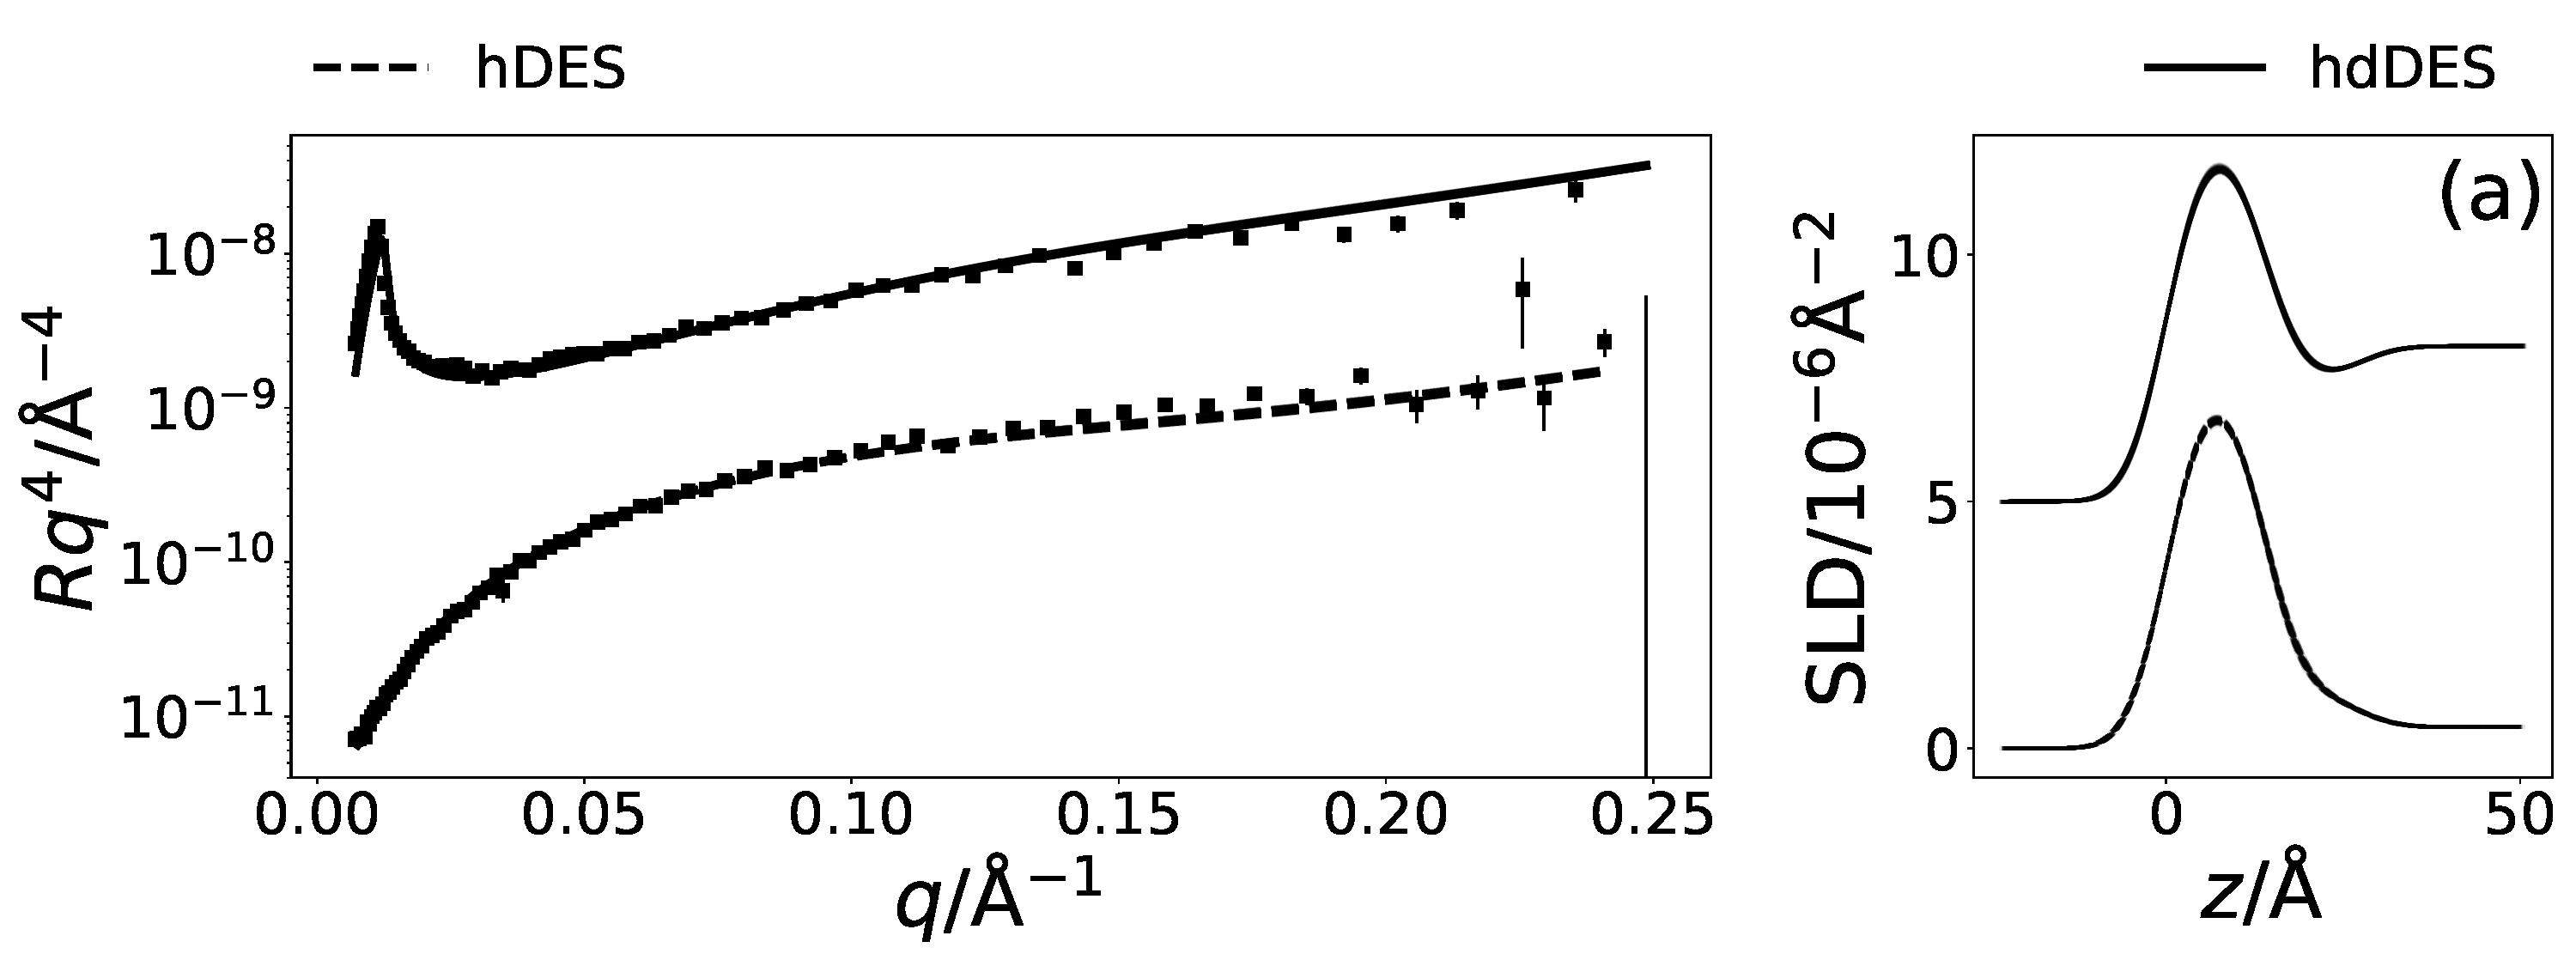
\includegraphics[width=0.45\textwidth]{figures/dmpc_20n_ref_sld}
	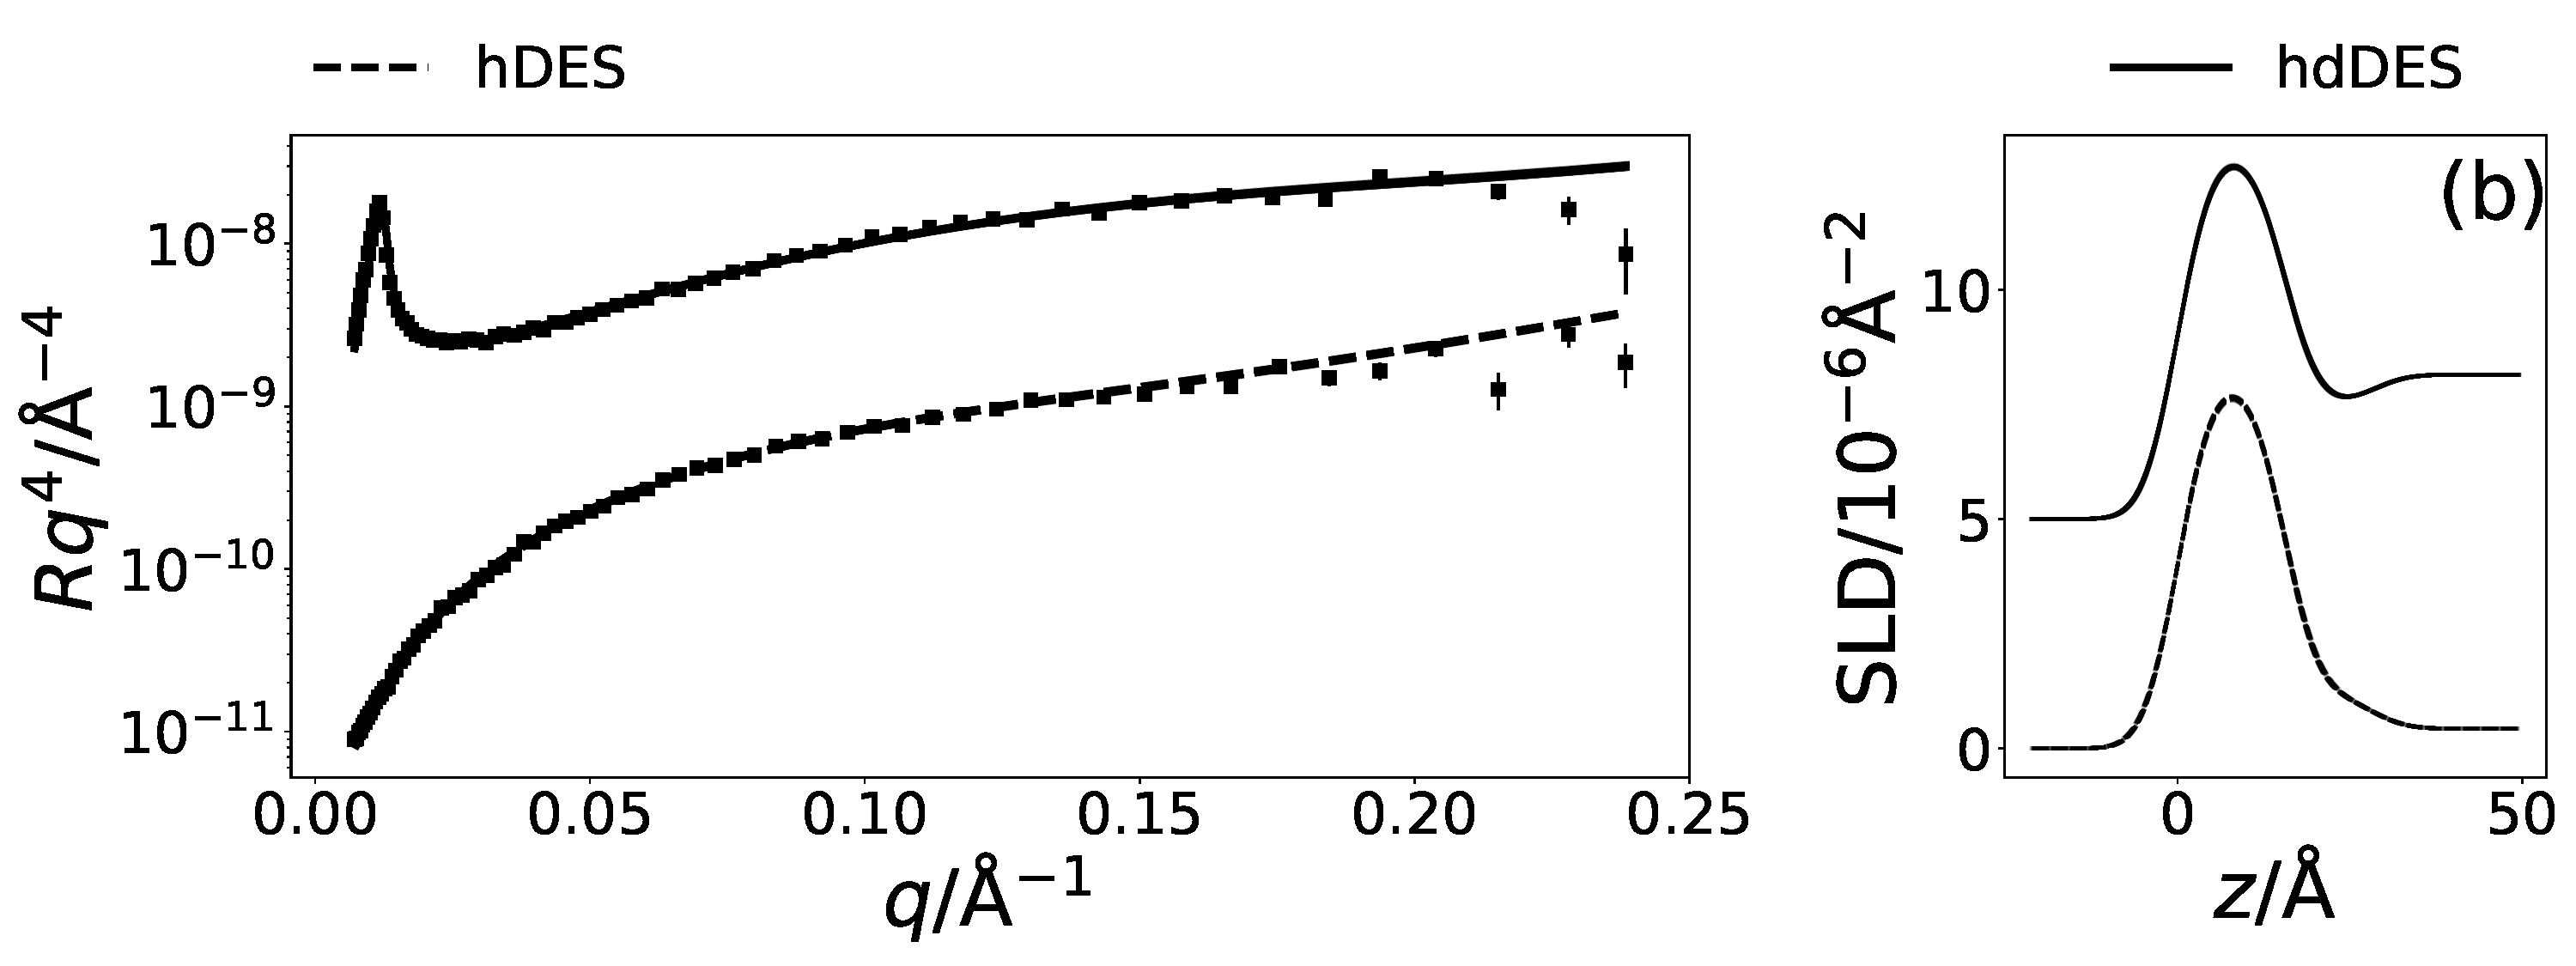
\includegraphics[width=0.45\textwidth]{figures/dppc_20n_ref_sld}
	\caption{\small The NR and SLD profiles at a surface pressure of 20 mNm$^{-1}$ for two contrasts (see legend above each plot); (a) DMPC, (b) DPPC. The NR profiles have been offset in the $y$-axis by an order of magnitude and SLD profiles offset in the $y$-axis by \SI{5e-6}{\per\square\angstrom}, for clarity.}
	\label{fig:neutron}
\end{figure}
%
%
\begin{table*}
  \centering
	\caption{\label{tab:neutron}\small The best-fit values, and associated 95 \% confidence intervals for the varying parameters in the co-refined NR models. The values of $d_t$ were found from the appropriate values of $\theta_t$ using Eqn. \ref{equ:tl}, and the values of $\phi_h$ were found using Eqn. \ref{equ:phih}.}
	\begin{tabular}{ccccc}
    Lipid & \multicolumn{2}{c}{d$_{54}$-DMPC} & \multicolumn{2}{c}{d$_{62}$-DPPC} \\
    SP/mNm$^{-1}$ & 20 & 25 & 15 & 20 \\
		\hline
		$\theta_t$/$^\circ$ & \input{../output/dmpc/angle20_neutron.txt} & \input{../output/dmpc/angle25_neutron.txt} & \input{../output/dppc/angle15_neutron.txt} & \input{../output/dppc/angle20_neutron.txt} \\
		$\sigma_{t,h,s}$/\AA & \input{../output/dmpc/rough20_neutron.txt} & \input{../output/dmpc/rough25_neutron.txt} & \input{../output/dppc/rough15_neutron.txt} & \input{../output/dppc/rough20_neutron.txt} \\
    \hline
    $\phi_h$/$\times10^{-2}$ & \input{../output/dmpc/solh20_neutron.txt} & \input{../output/dmpc/solh25_neutron.txt} & \input{../output/dppc/solh15_neutron.txt} & \input{../output/dppc/solh20_neutron.txt} \\
		$d_t$/\AA & \input{../output/dmpc/tail20_neutron.txt} & \input{../output/dmpc/tail25_neutron.txt} & \input{../output/dppc/tail15_neutron.txt} & \input{../output/dppc/tail20_neutron.txt} \\
	\end{tabular}
\end{table*}
%

For the first time, stable phosphocholine and phosphatidylglycerol lipid monolayers have been observed and characterised on a non-aqueous liquid surface.
Until the emergence of ionic liquids and DES, only a limited number of molecular solvents exhibited the ability to promote self-assembly and, to the best of our knowledge, only water among those had demonstrated the formation of functional phospholipid monolayers at the air-liquid interface.

A physically and chemically constrained modelling approach and Bayesian analysis method was used to rationalise these measurements showing that the structures are remarkably similar at the air-DES interface to those previously observed at the air-water interface.
This has the important implication that DES therefore offers the possibility of performing studies of model membranes in the absence of water.
Such applications may include fundamental investigations of phospholipid monolayers in extreme environments (total or partial absence of water, cryogenic temperatures), protein membrane interactions and development of new technologies for drug delivery.
However, the fact remains that the PG lipid did show a significant difference; having a larger head volume than observed for the same system in water.
This shows that the transfer of lipids to a DES is not just a simple substitution of the subphase. In this specific case we have proposed an explanation based on unfolding of the PG head that is enabled by electrostatic screening of the head charges by the charged solvent.

The ability to determine the head volume was facilitated by access to easy to use, and open-source software that allowed for the straightforward use a custom, chemically-consistent model within the analysis of the XRR and NR measurements.
Futhermore, this work presents the first, to our knowledge, use of chemically-consistent parameterisation to co-refine XRR measurements at different surface concentrations.

\section*{Acknowledgments}

The authors thank Andrew Nelson for his help with the refnx software.
A.R.M. is grateful to the University of Bath and Diamond Light Source for co-funding a studentship (Studentship Number STU0149).
The authors thank the European Spallation Source and the University of Bath Alumni Fund for supporting A.S.-F.
We also thank Diamond Light Source (Experiment number SI10546-1) and Institut Laue-Langevin (DOI: \href{http://doi.org/10.5291/ILL-DATA.9-13-612}{10.5291/ILL-DATA.9-13-612}) for the awarded beamtime.

\setlength{\bibsep}{1pt}
\bibliography{bibi}% Produces the bibliography via BibTeX.
\bibliographystyle{rsc}
\end{document}
